\documentclass[12pt]{article}
\usepackage[utf8]{inputenc}
\usepackage{graphicx}
\usepackage{amsmath}
\usepackage[a4paper, total={7in, 10in}]{geometry}
\graphicspath{ {./../res/} }

\title{Nanoparticles size estimation throught Mie resonances}
\author{Neven Gentil}
\date{April 2022}

\begin{document}

\maketitle

\twocolumn

\section{Introduction}
Hello LaTeX World!
Hello, here is some text without a meaning. This text should show what a printed text will look like at this place.
If you read this text, you will get no information. Really? Is there no information? Is there.Hello LaTeX World!
Hello, here is some text without a meaning. This text should show what a printed text will look like at this place.
If you read this text, you will get no information. Really? Is there no information? Is there.
\begin{figure}[h]
    \centering
    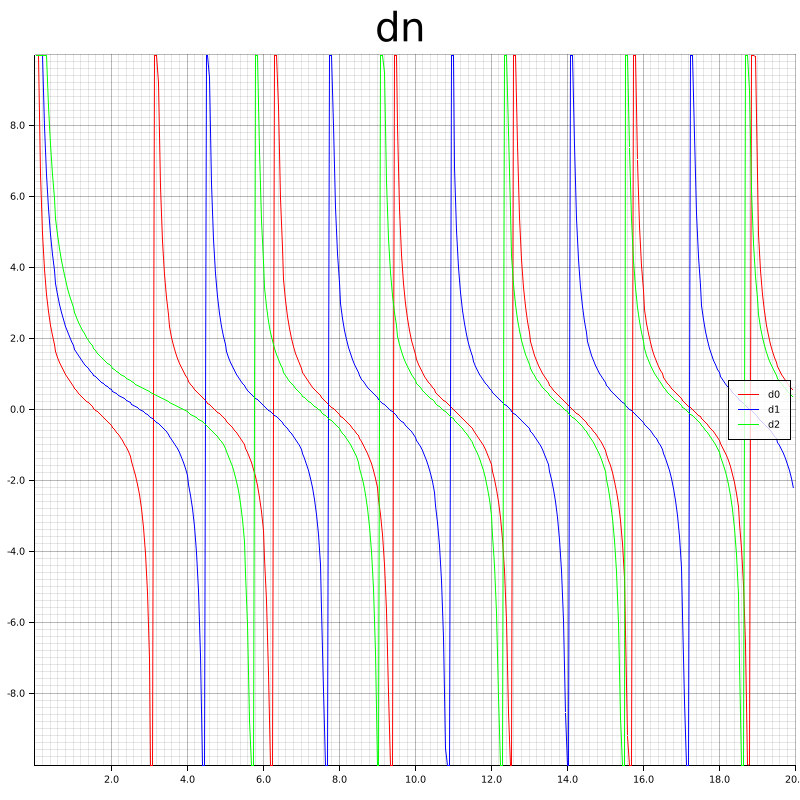
\includegraphics[width=0.5\textwidth, height=0.25\textheight]{dn.png}
    \caption{a nice plot}
    \label{fig:dn_plot}
\end{figure}
Hello LaTeX World!
Hello, here is some text without a meaning. This text should show what a printed text will look like at this place.
If you read this text, you will get no information. Really? Is there no information? Is there.Hello LaTeX World!
Hello, here is some text without a meaning. This text should show what a printed text will look like at this place.
If you read this text, you will get no information. Really? Is there no information? Is there.
\section{EXP}
\begin{figure}[h]
    \centering
    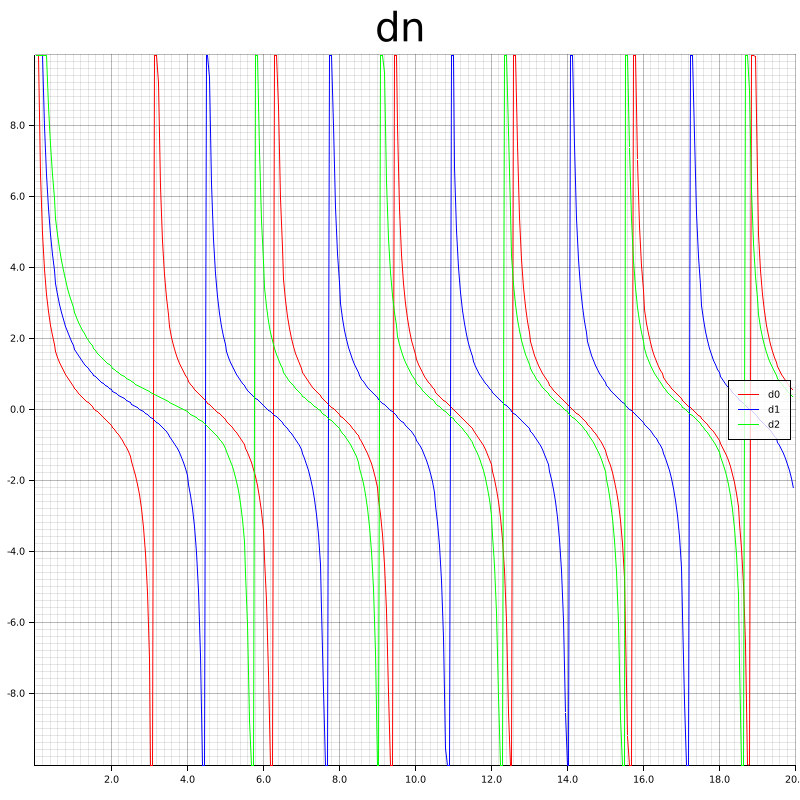
\includegraphics[width=0.5\textwidth, height=0.25\textheight]{dn.png}
    \caption{a nice plot}
    \label{fig:dn_plot}
\end{figure}
\begin{equation}
    \begin{aligned}
    E = m*2+4*x-4 / 5000.0 + 4000000 \\
    - 7777777 - 5 + 7777 + 4000000= 80a
\end{aligned}
\end{equation}
Hello LaTeX World!
Hello, here is some text without a meaning. This text should show what a printed text will look like at this place.
If you read this text, you will get no information. Really? Is there no information? Is there.Hello LaTeX World!
Hello, here is some text without a meaning. This text should show what a printed text will look like at this place.
If you read this text, you will get no information. Really? Is there no information? Is there.
Hello LaTeX World!
Hello, here is some text without a meaning. This text should show what a printed text will look like at this place.
If you read this text, you will get no information. Really? Is there no information? Is there.Hello LaTeX World!
Hello, here is some text without a meaning. This text should show what a printed text will look like at this place.
If you read this text, you will get no information. Really? Is there no information? Is there.
Hello LaTeX World!
Hello, here is some text without a meaning. This text should show what a printed text will look like at this place.
If you read this text, you will get no information. Really? Is there no information? Is there.Hello LaTeX World!
Hello, here is some text without a meaning. This text should show what a printed text will look like at this place.
If you read this text, you will get no information. Really? Is there no information? Is there.
Hello LaTeX World!
Hello, here is some text without a meaning. This text should show what a printed text will look like at this place.
If you read this text, you will get no information. Really? Is there no information? Is there.Hello LaTeX World!
Hello, here is some text without a meaning. This text should show what a printed text will look like at this place.
If you read this text, you will get no information. Really? Is there no information? Is there.

\newpage

\section{Introduction}

\section{Theorie}

\section{Simulations}

\section{Experiments}

\section{Conclusion}

\end{document}